
\documentclass[letterpaper, 10 pt, conference]{ieeeconf}  % Comment this line out
\usepackage{graphicx}
                                                          % if you need a4paper

\overrideIEEEmargins
% See the \addtolength command later in the file to balance the column lengths
% on the last page of the document

\usepackage[utf8]{inputenc}
\usepackage[T1]{fontenc}

% The following packages can be found on http:\\www.ctan.org
\usepackage{graphics} % for pdf, bitmapped graphics files
%\usepackage{epsfig} % for postscript graphics files
%\usepackage{mathptmx} % assumes new font selection scheme installed
%\usepackage{mathptmx} % assumes new font selection scheme installed
\usepackage{amsmath} % assumes amsmath package installed
\usepackage{amssymb}  % assumes amsmath package installed

\title{\LARGE \bf
Plantilla para informes de miniproyecto curso Técnicas de Deep Learning
}

\author{Nombre Autor 1 and Nombre Autor 2 }


\begin{document}

\maketitle
\thispagestyle{empty}
\pagestyle{empty}



%%%%%%%%%%%%%%%%%%%%%%%%%%%%%%%%%%%%%%%%%%%%%%%%%%%%%%%%%%%%%%%%%%%%%%%%%%%%%%%%
\section{Introducción}
En la introducción de un informe se debe presentar de manera clara el problema abordado, su relevancia y la contribución del trabajo. Para lograrlo, se recomienda comenzar con un contexto general que sitúe al lector en el área de estudio. Este puede incluir una breve referencia a los avances recientes y a su impacto en diversas aplicaciones, como visión por computadora, procesamiento del lenguaje natural o bioinformática. Además, es importante destacar los desafíos actuales.

Después de establecer el contexto, se debe definir con precisión el problema específico que se aborda en el informe. Es fundamental justificar su relevancia y explicar por qué representa un desafío dentro del campo. En este punto, es útil incluir referencias a estudios previos que han tratado de resolver problemas similares, resaltando sus limitaciones.

Finalmente, las introducciones finalizan con un pequeño párrafo especificando que se hizo en el estudio y cuales son los aportes del mismo. 


\section{Metodología}
La sección de metodología debe describir de manera detallada el enfoque propuesto. Es fundamental estructurar esta sección de forma clara y lógica, explicando los componentes clave del modelo, los datos utilizados y el procedimiento experimental.  

Se recomienda comenzar con una descripción general del enfoque seguido en el estudio. Aquí se puede proporcionar una visión global del método, resaltando sus principales características y cómo se diferencia de enfoques previos. En algunos casos, es útil incluir un diagrama que resuma la arquitectura del modelo o el flujo del proceso.  

A continuación, se deben detallar los datos utilizados en la investigación. Esto incluye la fuente de los datos, las características relevantes y cualquier preprocesamiento realizado. Es importante mencionar aspectos como la normalización de los datos, el aumento de datos o la división en conjuntos de entrenamiento, validación y prueba. 

Después de describir los datos, se debe presentar la arquitectura del modelo propuesto. En este apartado, se explica la estructura de la red neuronal o del algoritmo empleado, incluyendo el número de capas, los tipos de activaciones, las funciones de pérdida y los optimizadores utilizados.

Otro aspecto clave de la metodología es la estrategia de entrenamiento y evaluación. Aquí se deben especificar los hiperparámetros utilizados, como la tasa de aprendizaje, el tamaño del batch y el número de épocas. También se debe describir el procedimiento de validación, por ejemplo, si se utilizó validación cruzada o un conjunto de validación independiente. En cuanto a la evaluación del modelo, es esencial definir las métricas utilizadas (precisión, F1-score, IOU, etc.).

Finalmente, si se realizaron análisis adicionales, como estudios de ablación para evaluar la contribución de distintos componentes del modelo, estos también deben describirse en esta sección.  

\begin{figure}[h]
    \centering
    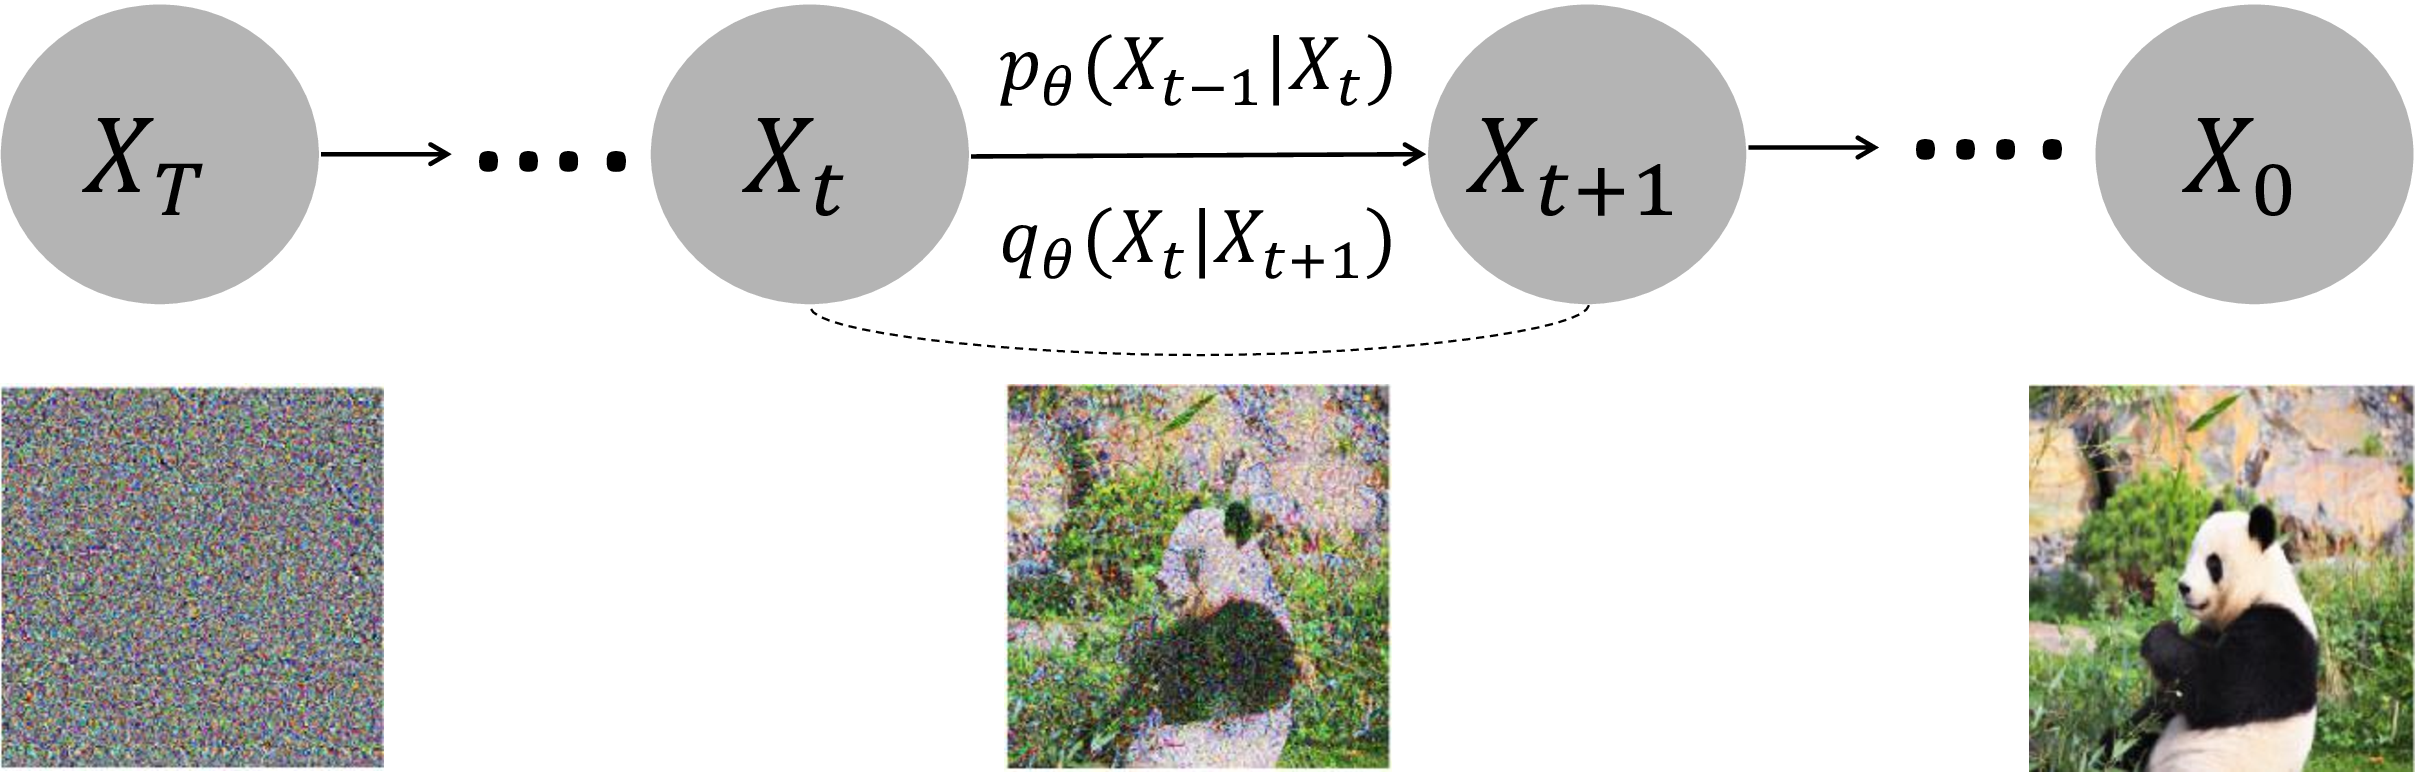
\includegraphics[width=0.95\linewidth]{Template_diffusion_models.png}
    \caption{Figura que ejemplifica un diagrama de la metodología de un paper que trabaja con modelos de difusión. Como se puede ver es un diagrama simple del funcionamiento del modelo utilizado. Es una práctica bastante común utilizar este tipo de diagramas para darle una idea al lector sobre cual fue el trabajo realizado.}
\end{figure}


\section{Resultados}

La sección de resultados en un informe se presenta y analiza los hallazgos obtenidos a partir de los experimentos realizados. Su objetivo es demostrar el desempeño del enfoque propuesto y, de ser posible, compararlo con otros métodos relevantes. Para que esta sección sea clara y efectiva, es recomendable estructurarla de manera ordenada, destacando los aspectos más relevantes de los resultados sin sobrecargar al lector con información innecesaria.

Se puede comenzar con una descripción general de los experimentos realizados y sus objetivos. Es importante recordar al lector qué aspectos del modelo se están evaluando y qué se espera demostrar con los resultados. En este punto, se pueden incluir\textbf{tablas} o \textbf{gráficos} que resuman las métricas clave obtenidas, como precisión, F1-score, pérdida, IoU, entre otras, dependiendo de la naturaleza del problema. Luego, se presentan los resultados cuantitativos obtenidos. 

Además de los resultados numéricos, es recomendable incluir análisis cualitativos cuando sea pertinente. En problemas como visión por computadora o generación de texto, las visualizaciones juegan un papel clave. Por ejemplo, en tareas de segmentación de imágenes, se pueden incluir ejemplos de segmentaciones predichas frente a las etiquetas reales para ilustrar el desempeño del modelo. En tareas de generación, se pueden presentar ejemplos de las muestras generadas y compararlas con ejemplos reales o con los resultados de otros modelos.

Otro aspecto importante son estudios de ablación para evaluar la contribución de diferentes componentes del modelo, análisis de sensibilidad a los hiperparámetros o evaluación en conjuntos de datos externos para probar la capacidad de generalización.

Finalmente, se debe proporcionar una interpretación de los resultados obtenidos. No basta con presentar métricas, sino que es clave explicar qué significan en el contexto del problema estudiado. Se pueden discutir implicaciones prácticas, limitaciones del enfoque y posibles mejoras futuras.

La sección de resultados debe ser clara y precisa, evitando interpretaciones especulativas sin evidencia experimental. Es recomendable apoyarse en figuras y tablas bien diseñadas para facilitar la comprensión de los hallazgos y permitir comparaciones efectivas.

\begin{table}[]
\centering
\caption{Ejemplo de una matriz de confusión en la que se presentan los resultados de un modelo de clasificación de imágenes.}
\resizebox{8.5cm}{!}{
\begin{tabular}{|c|c|c|c|} \hline
{\textbf{Pred vs }}{\textbf{Anot}}
& \textbf{Pulmón sano} & \textbf{Adenocarcinoma} & \textbf{Cel.Escamosas}\\\hline
\textbf{Pulmón sano} & 888 & 17 & 0 \\\hline
\textbf{Adenocarcinoma} & 112 & 837 & 140 \\\hline
\textbf{Cel. escamosas} & 0 & 146 & 860 \\\hline
\end{tabular}}
\end{table}

\section{Discusión}

La sección de discusión tiene como objetivo interpretar y contextualizar los resultados obtenidos, explicando su relevancia, implicaciones y posibles limitaciones. En esta sección, se analizan los hallazgos en profundidad y se relacionan con trabajos previos, destacando las contribuciones del estudio y proponiendo direcciones futuras.

Se puede comenzar con un resumen de los principales resultados obtenidos, resaltando los aspectos en los que el enfoque propuesto ha demostrado ser exitoso. Es importante contextualizar estos hallazgos dentro del campo de estudio y explicar cómo se comparan con investigaciones previas.

A continuación, es fundamental analizar las limitaciones del estudio. Todo modelo de Inteligencia Artificial tiene restricciones, y reconocerlas demuestra rigor científico. Estas limitaciones pueden estar relacionadas con la cantidad y calidad de los datos utilizados, la capacidad de generalización del modelo, el costo computacional del entrenamiento o la sensibilidad a ciertos hiperparámetros. También es relevante discutir posibles sesgos en los datos o en la metodología que podrían haber afectado los resultados.

% Para la parte de referencias puedes usar un archivo .bib o seguir el formato que convenga

\begin{thebibliography}{99}

\bibitem{c1} G. O. Young, ``Synthetic structure of industrial plastics (Book style with paper title and editor),'' 	in Plastics, 2nd ed. vol. 3, J. Peters, Ed.  New York: McGraw-Hill, 1964, pp. 15--64.
\bibitem{c2} W.-K. Chen, Linear Networks and Systems (Book style).	Belmont, CA: Wadsworth, 1993, pp. 123--135.
\bibitem{c3} H. Poor, An Introduction to Signal Detection and Estimation.   New York: Springer-Verlag, 1985, ch. 4.

\end{thebibliography}




\end{document}
